\chapter{Wing Lift Characteristics}
\label{ch:worklift}
\markboth{Wing Lift Characteristics}{}

\begin{flushright}
	{\smaller
		\textit{C'è qualcuno che può rompere il muro del suono,\\ mentre tutto il mondo si commenta da solo.}\\
		-- L. Ligabue}
\end{flushright}


Any body in motion in a fluid presents a result of force acting on it, which can be decomposed in two components:
\begin{itemize}
\item A {\bfseries Lift} acting normal to the Velocity direction and is positive upward.
\item A {\bfseries Drag} acting in the opposite direction to the airspeed vector.
\end{itemize}
The lifting surfaces of an airplane are designed to generate lift exceeding their drag, in order to obtain a positive efficiency. \\ In this chapter it will be explained how it is possible to evaluate the complete lift coefficient curve of a wing, both in its linear trait and non linear.\\
The lift coefficient is a dimensionless number used to model all of the complex dependencies of shape, inclination, and some flow conditions on lift. The lift coefficient also contains the effects of air viscosity and compressibility that are molded respectively with the Raynolds and Mach number.% [ Cap. \cite{nasaLift}] 

\section{Theoretical background}

In order to achieve the complete curve of coefficient list it is necessary to obtain the following parameters:

\begin{enumerate}
\item Zero-Lift Angle
\item Lift Coefficient slope 
\item End of Linearity Angle
\item Maximum Lift Coefficient
\item Stall Angle of attack
\end{enumerate}

Following it will be explained the theory behind how these contributions have been made.

\subsection{Zero-Lift Angle and Lift Coefficient Slope}

In order to evaluate the linear trait of the wing lift curve, it is been used the Nasa-Blackwell method.\\ The {\bfseries Nasa-Blackwell} is a numerical method for calculating the subsonic load distribution for arbitrary lifting surface arrangements at a fixed angle of attack. The method is suitable for swept wings, non-planar wings, wing with pylons and/or end-plates; it can be also used to study the aerodynamic interaction of the wing and the horizontal tail. The method has been implemented because its results, as shown in the report, were in good agreement with the experimental results.
The lifting surfaces are divided in several rectangular horse-shoe vortices along the span; one horseshoe vortex along the chord is used, that is, the midpoints of the vortices are placed only at points along the quarter-chord lines. An equal number of control points are located along the three-quarter-chord lines. The velocity from the total vortex system is equated to the component of free-stream velocity normal to the lifting surface chord at each control point. Application of this tangent-flow boundary condition for a symmetrical loading provides a set of N simultaneous equations in the N unknown circulation strengths. Solution of this set of equations provides the loading distributions over the lifting surfaces. Mach number effect is introduced through a Prandtl-Glauert correction. Further details can be found in \cite{NASA:Blackwell}.

In this way  the Zero Lift angle it is calculated using the integral of the load distribution and the linear trait slope starting from the value of CL at $\alpha =  0^{\circ}$ and $\alpha = 2^{\circ}$.

\begin{equation}
CL_{\alpha}= \frac{CL|_2 - CL|_0}{\upDelta \alpha}
\end{equation}

In JPAD it is possible also evaluating these two contributes using different methods. \\
For the evaluation of the $\alpha_{0L}$ it is possible to use a method of the class \texttt{CalcAlpha0L}, a nested class  in \texttt{LSAerodynamicManager}. Using these method, the zero-lift angle is calculated with the following formula, where $\epsilon_T$ is the twist angle:

\begin{equation}
\alpha_{0L} = \frac{1}{S}\int_{-\frac{b}{2}}^{\frac{b}{2}} c(y) [ \alpha_0(y) - \epsilon_T(y) ] \, dy
\end{equation}

This formula  is applied to the exposed wing. When a default aricraft is defined, during the creation of components, is calculated the exposed wing. This is the wing outside of the fuselage. It starts at semi-diameter of fuselage and its root airfoil is the airfoil of wing  at this station calculated by the method \texttt{calculateIntermediateAirfoil}.\\ \\

In order to evaluate the lift coefficient linear slope  it is possible to use different method belonging to \texttt{CalcCLAlpha} class. The first one use the Polhamus formula which is valid for arbitrary aspect ratios and sweep angles in subsonic flow:

\begin{equation}
CL_{\alpha} = \frac{2 \pi \AR}{ \left\{ 2 + \sqrt{\frac{\AR^2 \beta^2}{k^2} \left ( 1 + \frac{\tan^2{(\Lambda_{\frac{c}{2}})}}{\beta^2} \right) + 4 }\right\}}
\end{equation}

Thus $CL_{\alpha}$  is a function of wing aspect ratio, mid-chord sweep angle $\Lambda_{\frac{c}{2}}$, Mach number, and airfoil section (defined parallel to the free stream) lift curve slope. The factor K in the equation is the ratio of the experimental two-dimensional lift curve slope.\\
Alternately it is possible to use the Anderson formula for swept wing, compressible and subsonic flow:

\begin{equation}
CL_{\alpha} = 
\frac{Cl_{\alpha} \cos{\Lambda_{\frac{c}{2}}}}
{\sqrt{1 - M^2  cos^2 {\Lambda_{\frac{c}{2}}}
 + \left[ \frac{Cl_{\alpha} \cos{\Lambda_{\frac{c}{2}}}}{\pi \AR}\right]^2} + \frac{Cl_{\alpha} \cos{\Lambda_{\frac{c}{2}}}}{\pi \AR}}
\end{equation}



\subsection{End of Linearity angle of attack}

The angle of end linearity is calculated using the characteristics of the mean airfoil of the wing. This is obtained through the influence area of the airfoils as shown in fig. \ref{fig:influencearea}.

\begin{figure}[H]
\centering
{\includegraphics[height=3cm]{Immagini/influencearea}} 
\caption{Influence area of the sections for finite wing.}
\label{fig:influencearea}
\end{figure}

Then is possible to calculate the influence coefficients. 

\begin{equation}
K_i = \frac{2 S_i}{S}
\end{equation}

The mean parameters can be obtained from:

\begin{equation}
\overline{x} = x_1 K_1 + x_2 k_2 +x_3 k_3...
\end{equation}

In particular, for a wing defined by three airfoils, the end of linearity angle of attack is obtained from the following equation:

\begin{equation}
\alpha^* = \alpha^*_{1} K_1 + \alpha^*_{2} k_2 +\alpha^*_{3} k_3
\end{equation}

\subsection{Maximum Lift Coefficient}

In order to evauate the maximum lift coefficient the Stall Path Method has been used. The load distribution is calculated using Nasa-Blackwell method.

\begin{figure}[H]
\centering
{\includegraphics[height=6cm]{Immagini/Loading_Stall_Path_A}} 
\caption{Determination of wing lift distribution and Cl distribution of airfoils.}
\label{fig:stall0}
\end{figure}




The  practiced procedure is the following:

\begin{enumerate}
\item For each value of an Alpha array the load distribution is calculated using the NasaBlack method.  The distribution of  $Cl_{max}$ is known. fig. \ref{fig:stall1}.
\item At $\alpha = \alpha_j$ the load distribution curve intersects for the first time the $Cl_{max}$ curve of the airfoils. fig. \ref{fig:stall1}.
\item For each $ y > y_1 $ , along y axis (where y_1 is the station of first intersection) is evaluated the difference between $CL_{wing}$ and $Cl_{max}$. fig. \ref{fig:stall2}.
\item $\upDelta \alpha$ is evaluated until the maximum difference between $CL_{wing}$ and $Cl_{max}$ is smaller than the required accuracy. Actually the accuracy is 0.0001. 
\end{enumerate}

The evauation of $\upDelta \alpha$ is not simple.\\
After finding the first value of intersection between $CL_{wing}$ and $Cl_{max}$ a new $\alpha$ is evaluated. The first value used for the optimization is 

\begin{equation}\notag
\upDelta \alpha = \alpha_j -\alpha_{j-1}
\end{equation}
\begin{equation}\notag
\alpha_{new} = \alpha_j - \frac {\upDelta \alpha }{2}
\end{equation}
\begin{equation}\notag
\alpha_{old}= \alpha_j
\end{equation}

For the following step if there isn't a point of intersection at $\alpha_{new}$ the new value of $\alpha$ is, for the step $j+1$:


\begin{equation}\notag
\upDelta \alpha = |\alpha_{j-1} -\alpha_{j}|
\end{equation}
\begin{equation}\notag
\alpha_{new} = \alpha_{j} + \frac {\upDelta \alpha }{2}
\end{equation}
\begin{equation}\notag
\alpha_{old}= \alpha_j
\end{equation}

Instead,  if there is a point of intersection at $\alpha_{new}$ the new value of $\alpha$ is, for the step $j+1$:


\begin{equation}\notag
\upDelta \alpha =  |\alpha_{j-1} -\alpha_{j}|
\end{equation}
\begin{equation}\notag
\alpha_{new} = \alpha_{j} - \frac {\upDelta \alpha }{2}
\end{equation}
\begin{equation}\notag
\alpha_{old} = \alpha_j
\end{equation}



\begin{figure}[H]
\centering
{\includegraphics[height=6cm]{Immagini/Loading_Stall_Path_B}} 
\caption{Determination of wing lift distribution and Cl distribution of airfoils.}
\label{fig:stall1}
\end{figure}


\begin{figure}[H]
\centering
{\includegraphics[height=6cm]{Immagini/Loading_Stall_Path_D}} 
\caption{Intersection  between $CL_{wing}$ and $Cl_{max}$ curves.}
\label{fig:stall2}
\end{figure}

\begin{figure}[H]
\centering
{\includegraphics[height=6cm]{Immagini/Loading_Stall_Path_E}} 
\caption{Determination of $\upDelta \alpha$.}
\label{fig:stall5}
\end{figure}

\begin{figure}[H]
\centering
{\includegraphics[height=8.3cm]{Immagini/wing_loading_B}} 
\caption{Wing Loading distribution.}
\label{fig:wl}
\end{figure}

\subsection{Stall Angle of Attack}

Nasa-Blackwell is an inviscid method for calculating the subsonic aerodynamic load distributions for arbitrary lifting-surface arrangements. This means that it does not see the non linear trait of the lift curve. So in correspondence of the value of $C_{L_{MAX}}$ calculated, the angle of attack obtained from the Nasa-Blackwell method is not correct because it is the maximum angle of attack that you would get if you reach the max $C_L$ linearly.\\
So first it is evaluated the angle of attack at maximum lift coefficient through the linear trend of the lift line, then it’s added to this angle the increment evaluated by the diagram in fig. \ref{fig:dealpha}, this is valid strictly for wing with high taper ratio without twist, with unique airfoil type and Mach number included between 0.2 and 0.6.


\begin{figure}[H]
\centering
{\includegraphics[height=6.3cm]{Immagini/deltaAlphaSforza.png}} 
\caption{Diagram useful for evaluation of $\upDelta \alpha$.}
\label{fig:dealpha}
\end{figure}



\subsection{Construction of the curve}
At this point all elements are available in order to draft the CL vs $\alpha$ curve.\\ The linear trait is evaluated using the equation of straight line.

\begin{equation}
C_L= C_{L_\alpha} \alpha + C_{L_0}
\end{equation}

%There is a method in \texttt{LSAerodynamicManager} that evaluates the linear slope of lift curve of a lifting surface using Nasa-Blackwell method. This method ( \texttt{nasaBlackwell} in the nested class\texttt{CalcCLAlpha()} evaluate CL wing in correspondence of two alpha and calculates the angolar coefficient.

In order to plot the non linear trait is used a cubic function. In fact in this zone we have four conditions:

\begin{itemize}
\item Pass to $\alpha^{\star}$ , $C_L^{\star}$
\item The derivatine in  $\alpha^{\star}$ , $C_L^{\star}$ is $C_{L_\alpha}$ for continuity
\item Pass to $\alpha_{stall}$ , $C_{L_{MAX}}$
\item The derivatine in  $\alpha_{stall}$ , $C_{L_{MAX}}$ is $0$.Here there is the maximum of the curve.
\end{itemize}

So the system of equations is :

\begin{equation}
\begin{cases}
 C_L^{\star} = a {\alpha^{\star}}^3 +  b {\alpha^{\star}}^2 +  c {\alpha^{\star}} + d \\
 C_{L_\alpha} = 3 a {\alpha^{\star}}^2 +  2b {\alpha^{\star}} +  c  \\ 
 C_{L_{MAX}} = a {\alpha_{stall}}^3 +  b {\alpha_{stall}}^2 +  c {\alpha_{stall}} + d \\
0 = 3 a {\alpha_{stall}}^2 +  2b {\alpha_{stall}} +  c  \\ 
  \end{cases}
\end{equation}



\begin{figure}[H]
\centering
{\includegraphics[height=8.69cm]{Immagini/Wing_CL_Vs_alpha_curve.pdf}} 
\caption{Wing $C_L$ vs $\alpha$ curve.}
\label{fig:clalfa}
\end{figure}


%The method that draws the curve is \texttt{plotCLvsAlphaCurve()} in \texttt{LSAerodynamicsManager}.\\
%The method \texttt{plotCLvsAlphaCurve()} solves the system and calculates the parameters using a static function of \texttt{MyMathUtils}, \texttt{solveLinearSystem}.

\subsection{Mach number effects on Lift curve }
The features of airflow depend heavily from the Mach number. These changes in airflow have a significant effect on the airplane lift. For airplanes that operate entirely within the subsonic speed range, there are no significant effects of compressibility of the air on the airplane lift. For airplanes that operate at high subsonic speeds in the transonic speed region, the airplane lift and drag curves will vary as the flight Mach number is increased due to the compressible nature of the air, so there is a family of lift curves one for each flight Mach number of interest.\\
The family of lift curves is characterized by an increase in the slope of the curve and decrease in maximum lift coefficient as the Mach number increased in the high subsonic region as shown in the fig. \ref{fig:clalfawing}.
The explanation of these Mach number effects on the lift curve has been derived from the theory of compressible flow, and confirmed by experimental data obtained in wind tunnels and from flight tests. It can be shown that, for an airplane at given angle of attack, the lift coefficient will increase with Mach number because the suction on the wing upper surfac, and the pressures on the wing lower surface tend to grow with Mach number.  \cite{manual}

\begin{figure}[H]
\centering
{\includegraphics[height=5.6cm]{Immagini/clamach}} 
\caption{Mach number effects on Lift curve.}
\label{fig:clalfawing}
\end{figure}

\begin{figure}[H]
\centering
{\includegraphics[height=5.6cm]{Immagini/declmach.png}} 
\caption{Mach number effects on Lift linear slope.}
\label{fig:clalfawingslope}
\end{figure}

\subsection{High Lift devices}
The aircraft’s performances at low speed are very important for their mission, infact good high lift devices allow to land or take off on many airports, with their various runways.\cite{adas}
To assure high lift in take-off and landing without varying weight and wing surface, it is varied the airfoil shape, for this reasons high-lift systems are used. High-lift systems are commonly defined as the devices that allow to increase the maximum lift coefficient of the aircraft and consequently to decrease the stalling speeds. 
A great variety of high lift devices exists, many of which are mechanically complex. The most simple systems change only the camber of the aerofoil. More complex concepts not only change camber but also extend the chord, opening up slots as they do so. \cite{howe2000aircraft}\\
High-lift devices can be classified in two main categories: trailing edge devices, or leading edge devices.
TE devices are small aerofoil-like elements that are fitted at the trailing edge of the wing that are called flap, while  at the LE as a slat.


\begin{figure}[H]
\centering
{\includegraphics[height=11.3cm, angle =-90 ]{Immagini/highlift.png}} 
\caption{Different kind of High Lift devices and their effects.}
\label{fig:hl}
\end{figure}

In order to evaluate the new wing lift curve with flap and slat it is necessary to evaluate the contribution due to these devices starting from the clean $C_L$ vs $\alpha$ curve. In particular these contributions on the lift curve are the following:

\begin{itemize}
\item $\upDelta C_{L_0} $ flap 
\item $\upDelta C_{L_{MAX}} $ flap
\item $CL_{\alpha}$ flap 
\item $\upDelta \alpha_{MAX} $ flap
\item $\upDelta C_{L_{MAX}} $ slat
\item $\upDelta \alpha_{MAX} $ slat
\end{itemize}


All of these parameters are calculated using formulas or graphs. For further details see \cite{nicolai2010fundamentals}

\begin{figure}[H]
\centering
{\includegraphics[height=12.9cm]{Immagini/Airfoil_Cl_Vs_alpha_curve_flap_slat.pdf}} 
\caption{Wing $C_L$ vs $\alpha$ curve for clean wing and with high lift devices.}
\label{fig:clalfahl}
\end{figure}


\section{Java Class Architecture}

In this paragraph the implementation inside the JPAD library of the calculation of the wing lift characteristics will be described. In JPAD there are several methods relating to the calculation of lift or wing load, which are summarized in the table below, all contained in \texttt{LSAerodynamicManager} class. In order to have a clear organization of the class, the methods relating to the calculations of the same items are organized in nested classes.

\begin{table}[H]
\begin{tabular}{p{7cm}p{7.5cm}}
\toprule
\lstinline[language=Java]!CalcBasicLoad! & This nested class contains a method that evaluate the basic load semi-spanwise using the Schrenk method.\\ \hline 
\lstinline[language=Java]!CalcLiftDistribution! &This nested class contains some methods that calculates the lift distribution semi-spanwise. It is possible to choose Schrenk method, the Nasa-Blackwell method and it is also possible to evaluate the lift distibution using 50 airfoil and evaluating for each of them the lift coefficient from the 2D lift curves. \\ \hline 
\lstinline[language=Java]!CalcCLAtAlpha! & Using a method of this class it is possible to evaluate the lift coefficient of a lifting surface at a given angle of attack. It is possible to use the following formulas: DLR equation, Anderson compressible subsonic equation and Nasa-Blackwell method. With the last method it is calculated both linear trait and non linear trait. In order to builds the non-linear trait a cubic interpolation is used.\\ \hline 
\lstinline[language=Java]!CalcCLMaxClean! &This class contains some method that evaluatex the maximum lift coefficient of a lifting surface without hig-lift devices. It' possible to use Phillips and Alley method or stall path method in which the load distribution in evaluated with Nasa-Blackwell method.\\ \hline 
\lstinline[language=Java]!plotCLvsAlphaCurve()! & This function plot CL vs Alpha curve of an isolated wing using 30 value of alpha between $\alpha = - 10.0^{\circ}$  deg and  $\alpha = \alpha + 2^{\circ}$.\\ \hline 
\lstinline[language=Java]!CalcCLvsAlphaCurve!&The methods of this class, calculate CL at alpha given as input. It uses values of field filled before. So in order to evaluate the lift coefficient with this class it is necessary to call other method before.\\ \hline 
\lstinline[language=Java]!calcAlphaAndCLMax! & This method calls all the needed method in order to evaluate the maximum lift coefficient and the stall angle.\\ \hline 
\lstinline[language=Java]!CalcHighLiftDevices! & This method calculates the effects of high-lift devices on the lift characteristics.\\ \hline 
\lstinline[language=Java]!CalcCLAlpha! & This class calculates the lift coefficient gradient of the whole lifting surface. It is possible to choose Polhamus formula,  Anderson equation, or Nasa-Blackwell method where the lift coefficient gradient is evaluated from two value of lift coefficient.\\ \hline 
\lstinline[language=Java]!CalcCL0! & This class calculates $C_{L_0}$ using Anderson formula.\\ \hline 
\bottomrule
\end{tabular}
\caption{Methods for lift characteristcs of a lifting surface.}
\label{table:Table2}
\end{table}

In order to evaluate the lift coefficient of a lifting surface and to obtain the lift curve it is necessary, first of all, to define an object of \texttt{LSAerodynamicManager} class. This class holds all aerodynamic analysis methods available for a generic lifting surface. There are different constructors of this class depending on the presence of the aircraft. In fact in JPAD it is possible to analyze a complete aircraft or an isolated wing. In both cases it is necessary to give an object of \texttt{OperatingConditions} class as input parameter. After it is possible to define an object of the nested class \texttt{CalcCLAtAlpha} and then it is possible to use a method of this class in order to evaluate the lift coefficient. The process is shown in Fig.\ref{fig:clalf}.

\begin{figure}[H]
\centering
{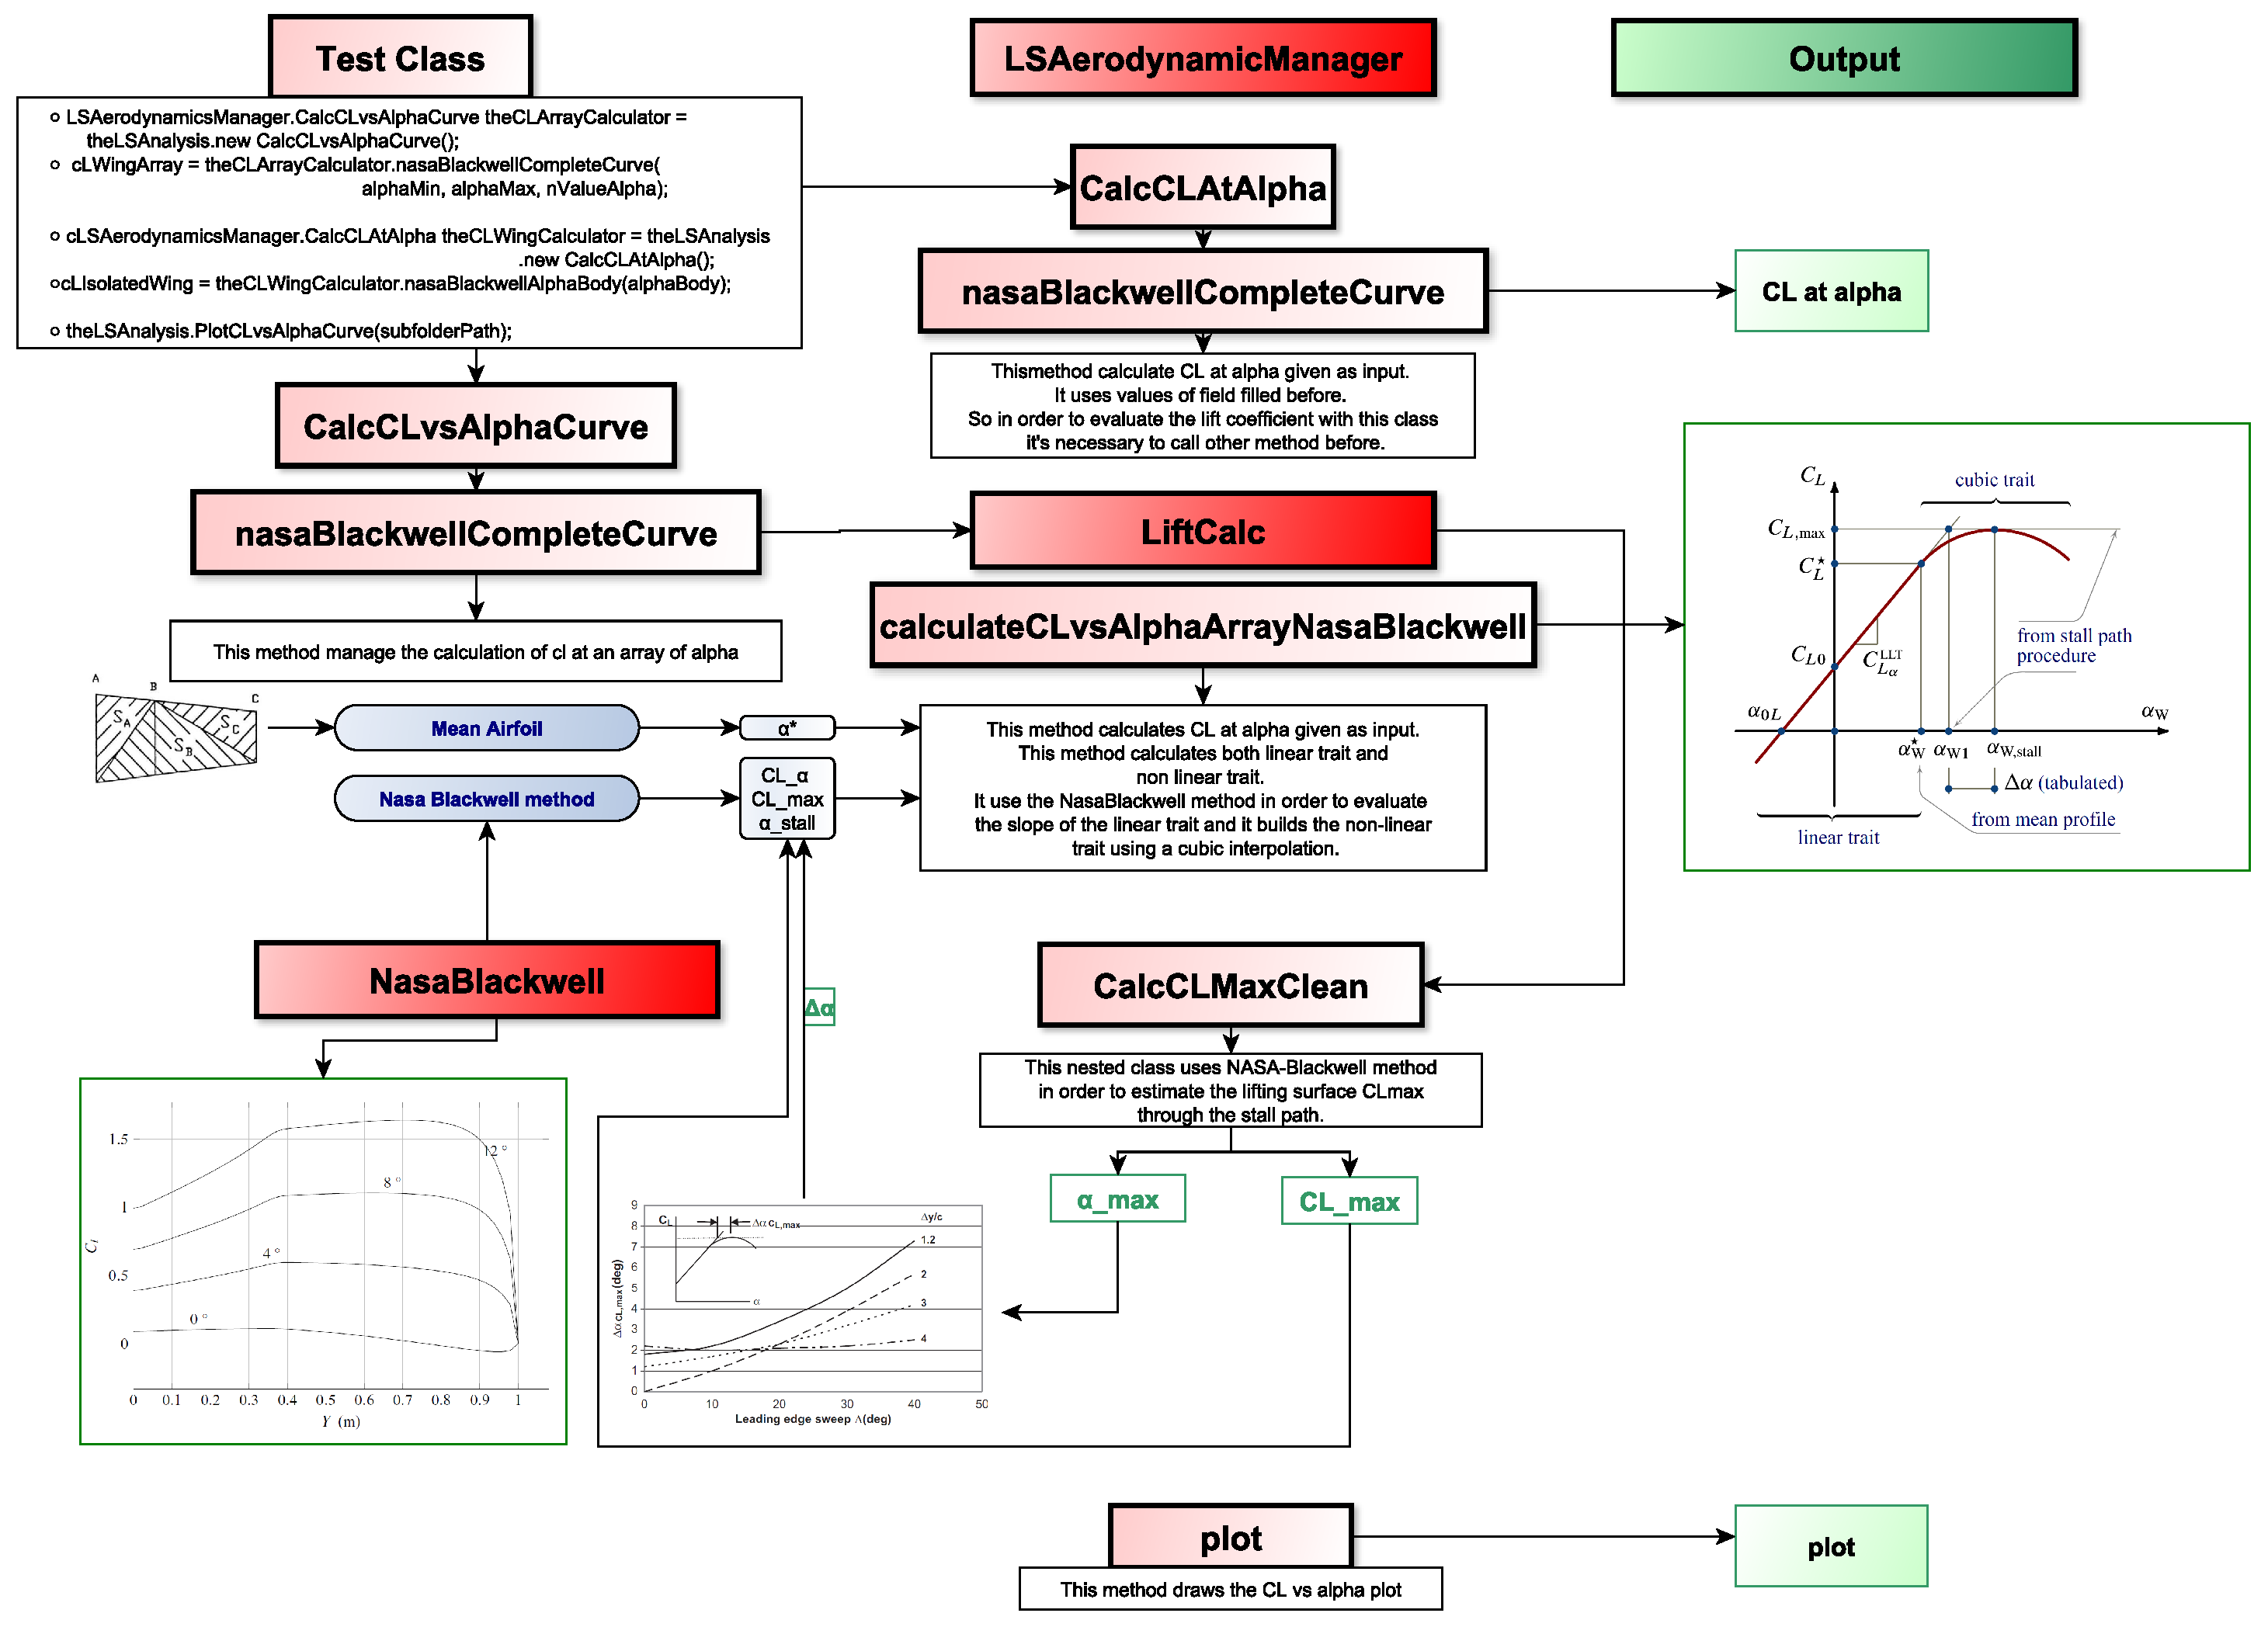
\includegraphics[height=14.6cm, angle=90]{Immagini/clflowchart.pdf}} 
\caption{Flow chart of lift estimation classes.}
\label{fig:clalf}
\end{figure}


\section{Case Study}

The last task to be done is to show an application of the calculation of lift characteristics of a lifting surface in order to validate the calculation performed as well as to give a useful example of use. In previous chapters two aircraft were introduced: ATR-72 and B747-100B. On these two aircrafts analyses were made, the results of which are shown below.\\

\subsection{ATR-72}

In order to correctly use the lift modulus of JPAD it is necessary to set the correct Reynolds number of airfoils and, consequently, the correct value of $CL_{MAX}$. Referring to \cite{Abbott} the value for ATR 72 are the following

\begin{center}
\captionof{table}{Airfoils $CL_{MAX}$ for ATR-72. Mach number = 0.4}
	\begin{tabular}{ | l | l | l | l |}
		\hline
		Station & Airfoil & Reynolds Number & $CL_{max}$ \\ \hline
		Root & NACA 23018 & $6.28 \cdot 10^6$ & 1.65 \\ \hline
		Kink & NACA 23018 &  $6.28 \cdot 10^6$ & 1.65 \\ \hline
		Tip & NACA 23015 & $4.41 \cdot 10^6$ & 1.7 \\
		\hline
	\end{tabular}
\end{center}


\begin{figure}[H]
	\centering
	{\includegraphics[height=6.8cm]{Immagini/ATR_Topview.pdf}} 
	\caption{Lift curve for ATR-72 airfoils and wing for M=0.2.}
	\label{fig:clalf}
\end{figure}

\begin{lstlisting}[frame=rbl,caption={{\footnotesize Lift Characteristics of a Lifting Surface - Test Class}},label= [style=\bfseries]{Listing}]

System.out.println("\n\n------------------------------------");
System.out.println("\n LIFT CHARACTERISTICS  ");
System.out.println("\n------------------------------------");


System.out.println("\n ------------------- ");
System.out.println("|       WING        |");
System.out.println(" ------------------- \n\n");

System.out.println("\n \t Data: ");

System.out.println("Angle of attack alpha body (deg) = "
		+ "" + Math.ceil(alphaBody.to(NonSI.DEGREE_ANGLE)
				.getEstimatedValue()));
System.out.println("Angle of incidence of wing (deg) = "
		+ "" +  Math.ceil(theWing.get_iw()
				.to(NonSI.DEGREE_ANGLE)
				.getEstimatedValue()));

System.out.println("\n \n-----------------------------------------------------");
System.out.println("Starting evaluate stall path of wing");
System.out.println("-----------------------------------------------------");

LSAerodynamicsManager theLSAnalysis = new LSAerodynamicsManager(
				theConditions,
				theWing,
				aircraft
				);
				
LSAerodynamicsManager.CalcCLAtAlpha theCLWingCalculator = 
				theLSAnalysis
				.new CalcCLAtAlpha();
cLIsolatedWing = theCLWingCalculator.nasaBlackwellalphaBody(alphaBody);

theLSAnalysis.PlotCLvsAlphaCurve(subfolderPath);
System.out.println("-------------------------------------");
System.out.println("CL of Isolated wing at alpha body = " + cLIsolatedWing);
System.out.println("\n \t \t \tDONE PLOTTING CL VS ALPHA CURVE  ");

// -----------------------------------------------------------------------
// Using NASA-Blackwell method in order to estimate the lifting surface CLmax
// -----------------------------------------------------------------------


LSAerodynamicsManager.CalcCLMaxClean theCLmaxAnalysis = 
		theLSAnalysis
		.new CalcCLMaxClean(); //is nested
LSAerodynamicsManager.CalcCLvsAlphaCurve theCLAnalysis
       = theLSAnalysis.new CalcCLvsAlphaCurve();
theCLAnalysis.nasaBlackwell();
theCLmaxAnalysis.nasaBlackwell();
Amount<Angle> alphaAtCLMax = theLSAnalysis.get_alphaStall();
double clMax = theCLWingCalculator.nasaBlackwell(alphaAtCLMax);


// PLOT

System.out.println("\n \n \t \t WRITING CHART TO FILE. Stall path. ");

// interpolation of CL MAX_airfoil
		MyArray clMaxAirfoil = theCLmaxAnalysis.getClAirfoils();

		MyArray clAlphaThird = theLSAnalysis.getcLMap()
				.getCxyVsAlphaTable()
				.get(MethodEnum.NASA_BLACKWELL ,alphaAtCLMax);

		double [][] semiSpanAd = {
				theLSAnalysis.get_yStationsND(),
				 theLSAnalysis.get_yStationsND()};

		double [][] clDistribution = {
				clMaxAirfoil.getRealVector().toArray(), 
				clAlphaThird.getRealVector().toArray()};
		String [] legend = new String [4];
		legend[0] = "CL max airfoil";
		legend[1] = "CL distribution at alpha " 
		+ Math.toDegrees( alphaAtCLMax.getEstimatedValue());


MyChartToFileUtils.plot(
		semiSpanAd,	clDistribution, // array to plot
		0.0, 1.0, 0.0, 2.0,					
		"eta", "CL", "", "",	    // label with unit
		legend,					// legend
		subfolderPath, "Stall Path of Wing ");			


System.out.println("-----------------------------------------------------");
System.out.println("\t \t DONE ");

\end{lstlisting}


\begin{lstlisting}[caption={{\footnotesize Lift Characteristics of a Lifting Surface - Results for M=0.2. ATR-72}},label= [style=\bfseries]{Listing}]
------------------------------------

 LIFT CHARACTERISTICS  

------------------------------------

 ------------------- 
|       WING        |
 ------------------- 
 	 Data: 
Angle of attack alpha body (deg) = 2.0
Angle of incidence of wing (deg) = 2.0

 
-----------------------------------------------------
Starting evaluate stall path of wing
-----------------------------------------------------

 -----------CLEAN-------------- 
 alpha max 15.229385456031025 (deg)
 alpha star 10.918671750781748 (deg)
 cL max 1.4880884199886235
 cL star 1.1785803287397512
 cL alpha 5.582578511036018 (1/rad)
-------------------------------------
CL of Isolated wing at alpha body = 0.5045422247468523

 	 	 	DONE PLOTTING CL VS ALPHA CURVE  

 
 	 	 WRITING CHART TO FILE. Stall path. 
-----------------------------------------------------
	 	 DONE 
\end{lstlisting}


\noindent \\

\begin{figure}[H]
\centering
\input{immagini/stallpathatr.tikz}
\caption{ATR 72 Stall Path of wing at Mach 0.2.}
\label{fig:stallATR}
\end{figure}


\begin{figure}[H]
\centering
%CL vs Alpha clean WING
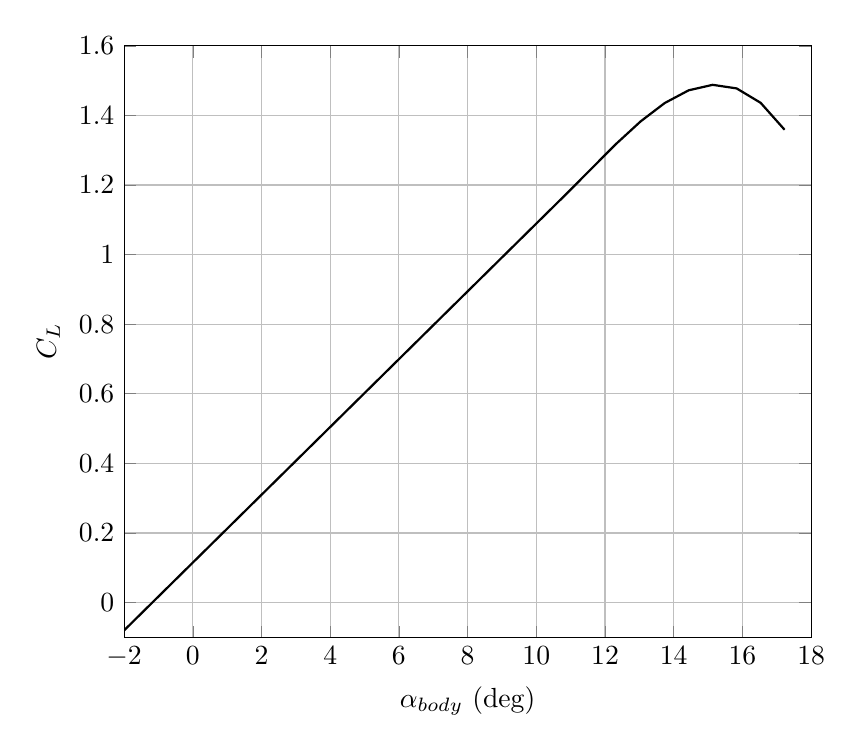
\begin{tikzpicture}

\begin{axis}[
width=0.85\textwidth,
height=0.75\textwidth,
scaled ticks=false, tick label style={/pgf/number format/fixed},
xmin=-2,
xmax=18,
xlabel={$\alpha_{body}$ (deg)},
xmajorgrids,
ymin=-0.1,
ymax=1.6,
ylabel={$C_L$ },
ymajorgrids,
]

\addplot [
color=black,
thick
]
table[row sep=crcr]{
-10.0	-0.8595390360144025\\
-9.30183939177138	-0.7915141929653783\\
-8.603678783542762	-0.723489349916354\\
-7.905518175314142	-0.6554645068673297\\
-7.207357567085522	-0.5874396638183055\\
-6.509196958856902	-0.519414820769281\\
-5.811036350628282	-0.4513899777202568\\
-5.112875742399662	-0.38336513467123234\\
-4.4147151341710416	-0.3153402916222081\\
-3.716554525942422	-0.24731544857318366\\
-3.0183939177138024	-0.17929060552415943\\
-2.320233309485183	-0.11126576247513506\\
-1.6220727012565632	-0.0432409194261108\\
-0.9239120930279435	0.024783923622913512\\
-0.22575148479932383	0.09280876667193784\\
0.47240912342929586	0.16083360972096217\\
1.1705697316579156	0.22885845276998645\\
1.8687303398865351	0.29688329581901074\\
2.5668909481151547	0.364908138868035\\
3.2650515563437743	0.43293298191705937\\
3.963212164572394	0.5009578249660838\\
4.6613727728010135	0.568982668015108\\
5.3595333810296335	0.6370075110641324\\
6.0576939892582535	0.7050323541131567\\
6.755854597486874	0.773057197162181\\
7.454015205715494	0.8410820402112054\\
8.152175813944114	0.9091068832602297\\
8.850336422172733	0.9771317263092539\\
9.548497030401352	1.0451565693582783\\
10.246657638629971	1.1131814124073025\\
10.94481824685859	1.1812096690481177\\
11.64297885508721	1.250789828512938\\
12.341139463315828	1.31974640200939\\
13.039300071544448	1.3830048566498019\\
13.737460679773067	1.43549065954651\\
14.435621288001686	1.472129277811844\\
15.133781896230305	1.4878461785581298\\
15.831942504458924	1.4775668288977095\\
16.530103112687545	1.436216695942909\\
17.228263720916168	1.3587212468060668\\
};
\end{axis}
\end{tikzpicture}%

\caption{ATR 72 CL vs Alpha_w at Mach 0.2.}
\label{fig:clATR}
\end{figure}

\begin{figure}[H]
\centering
%CL vs Alpha clean WING
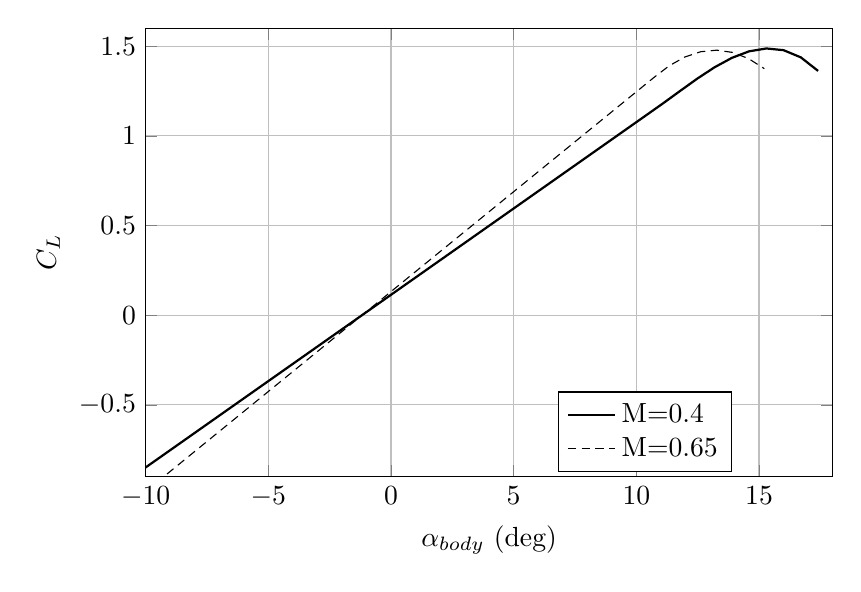
\begin{tikzpicture}

\begin{axis}[
width=0.85\textwidth,
height=0.6\textwidth,
scaled ticks=false, tick label style={/pgf/number format/fixed},
xmin=-10,
xmax=18,
xlabel={$\alpha_{body}$ (deg)},
xmajorgrids,
ymin=-0.9,
ymax=1.6,
ylabel={$C_L$ },
ymajorgrids,
legend style={at={(0.6,0.1)},anchor=west,draw=black,fill=white,legend cell align=left},
legend entries = {M=0.4\\M=0.65\\}
]

\addplot [
color=black,
thick
]
table[row sep=crcr]{
-10.0	-0.8492929893620671\\
-9.297278522952698	-0.7816396236505276\\
-8.594557045905397	-0.7139862579389877\\
-7.891835568858096	-0.6463328922274483\\
-7.189114091810795	-0.5786795265159088\\
-6.486392614763495	-0.5110261608043694\\
-5.783671137716194	-0.4433727950928297\\
-5.080949660668893	-0.37571942938129016\\
-4.378228183621593	-0.3080660636697507\\
-3.6755067065742915	-0.24041269795821102\\
-2.9727852295269903	-0.17275933224667145\\
-2.270063752479689	-0.10510596653513188\\
-1.567342275432388	-0.03745260082359231\\
-0.864620798385087	0.030200764887947262\\
-0.16189932133778595	0.09785413059948683\\
0.5408221557095151	0.1655074963110264\\
1.2435436327568161	0.233160862022566\\
1.9462651098041173	0.30081422773410554\\
2.6489865868514184	0.36846759344564517\\
3.3517080638987196	0.43612095915718474\\
4.05442954094602	0.5037743248687243\\
4.757151017993321	0.5714276905802638\\
5.459872495040622	0.6390810562918033\\
6.162593972087922	0.7067344220033429\\
6.865315449135223	0.7743877877148825\\
7.568036926182524	0.8420411534264218\\
8.270758403229825	0.9096945191379616\\
8.973479880277127	0.9773478848495011\\
9.676201357324429	1.0450012505610409\\
10.37892283437173	1.1126546162725803\\
11.081644311419032	1.18043691390843\\
11.784365788466333	1.2503228114740352\\
12.487087265513635	1.319267928049312\\
13.189808742560936	1.3823490591100178\\
13.892530219608238	1.4346430001319082\\
14.59525169665554	1.4712265465907404\\
15.297973173702841	1.48717649396227\\
16.00069465075014	1.4775696377222598\\
16.703416127797443	1.4374827733464635\\
17.40613760484474	1.361992696310633\\
};
\addplot [
color=black,
densely dashed
]
table[row sep=crcr]{
-10.0	-0.9830709498739174\\
-9.353404038062589	-0.9110197055897866\\
-8.706808076125178	-0.8389684613056556\\
-8.060212114187767	-0.7669172170215245\\
-7.413616152250356	-0.6948659727373936\\
-6.7670201903129445	-0.6228147284532626\\
-6.1204242283755335	-0.5507634841691317\\
-5.473828266438122	-0.47871223988500067\\
-4.827232304500711	-0.40666099560086966\\
-4.1806363425633	-0.33460975131673865\\
-3.534040380625889	-0.2625585070326078\\
-2.887444418688478	-0.19050726274847685\\
-2.240848456751067	-0.11845601846434581\\
-1.5942524948136558	-0.04640477418021485\\
-0.9476565328762449	0.025646470103916075\\
-0.30106057093883387	0.09769771438804703\\
0.3455353909985771	0.169748958672178\\
0.9921313529359881	0.24180020295630894\\
1.6387273148733992	0.3138514472404399\\
2.2853232768108103	0.38590269152457085\\
2.9319192387482214	0.4579539358087018\\
3.5785152006856324	0.5300051800928328\\
4.225111162623043	0.6020564243769637\\
4.871707124560454	0.6741076686610947\\
5.518303086497865	0.7461589129452257\\
6.164899048435276	0.8182101572293566\\
6.8114950103726875	0.8902614015134876\\
7.4580909723100985	0.9623126457976184\\
8.104686934247509	1.0343638900817496\\
8.75128289618492	1.1064151343658806\\
9.397878858122331	1.1784663786500114\\
10.044474820059742	1.2505176229341421\\
10.691070781997153	1.3225688672182734\\
11.337666743934564	1.390505200152445\\
11.984262705871975	1.439904417061328\\
12.630858667809386	1.4691032486904354\\
13.277454629746797	1.4776297707703807\\
13.924050591684209	1.4650120590317752\\
14.57064655362162	1.4307781892052334\\
15.217242515559029	1.3744562370213669\\
};
\end{axis}
\end{tikzpicture}%

\caption{ATR-72 lift curve. Variation with Mach number.}
\label{fig:clATR}
\end{figure}




\begin{center}
\captionof{table}{High-lift devices geometrical data for ATR72}
	\begin{tabular}{| l | l | l | l | l |}
	\hline
		 Number of Flap & Type &  $\eta$ in &  $\eta$ out &   $\frac{c_{f}}{c} $   \\ \hline
		1  & Single Slotted& 0.08  & 0.35 &  0.38 \\ \hline
		2  & Single Slotted& 0.35 & 0.8 & 0.38 \\ \hline
		\hline
	\end{tabular}
\end{center}


\begin{center}
\captionof{table}{High-lift devices data for ATR72}
	\begin{tabular}{ | l | l | l |}
		\hline
		Configuration &  $\delta_{f_1}$ & $\delta_{f_2}$  \\ \hline
		Take off &  $22^{\circ}$ &  $22^{\circ}$\\ \hline
		Landing  &  $40^{\circ}$ &  $40^{\circ}$\\ \hline
		\hline
	\end{tabular}
\end{center}



\begin{figure}[H]
\centering
%CL alpha Wing High Lift
\begin{tikzpicture}

\begin{axis}[
width=0.9\textwidth,
height=0.55\textheight,
scaled ticks=false, tick label style={/pgf/number format/fixed},
xmin=-14.0,
xmax=20,
xlabel={alpha ($\deg$)},
xmajorgrids,
ymin=-0.8595390360144025,
ymax=2.7,
ylabel={C\textsubscript{L}},
ymajorgrids,
legend entries = {Clean\\Flap@TO\\}
]

\addplot [
color=black,
densely dashed
]
table[row sep=crcr]{
-10.0	-0.7990169022409647\\
-9.244265130095556	-0.730565177361426\\
-8.488530260191112	-0.662113452481887\\
-7.732795390286668	-0.5936617276023484\\
-6.977060520382224	-0.5252100027228094\\
-6.22132565047778	-0.4567582778432707\\
-5.465590780573336	-0.38830655296373184\\
-4.709855910668892	-0.319854828084193\\
-3.9541210407644485	-0.2514031032046542\\
-3.1983861708600045	-0.18295137832511532\\
-2.4426513009555606	-0.11449965344557647\\
-1.6869164310511167	-0.04604792856603768\\
-0.9311815611466728	0.022403796313501145\\
-0.175446691242229	0.09085552119303995\\
0.5802881786622148	0.1593072460725788\\
1.3360230485666587	0.2277589709521176\\
2.0917579184711026	0.29621069583165643\\
2.8474927883755465	0.36466242071119526\\
3.6032276582799905	0.4331141455907341\\
4.358962528184434	0.5015658704702729\\
5.114697398088878	0.5700175953498117\\
5.870432267993322	0.6384693202293504\\
6.626167137897766	0.7069210451088894\\
7.38190200780221	0.7753727699884282\\
8.137636877706653	0.843824494867967\\
8.893371747611097	0.912276219747506\\
9.64910661751554	0.9807279446270446\\
10.404841487419985	1.0491796695065831\\
11.160576357324429	1.118003287133353\\
11.916311227228872	1.1913380917053247\\
12.672046097133316	1.2675498588842884\\
13.42778096703776	1.3430685741896835\\
14.183515836942204	1.4143242231409459\\
14.939250706846648	1.4777467912575113\\
15.694985576751092	1.5297662640588183\\
16.450720446655534	1.5668126270643028\\
17.20645531655998	1.5853158657934023\\
17.962190186464422	1.5817059657655537\\
18.717925056368866	1.5524129125001962\\
19.47365992627331	1.4938666915167658\\
};

\addplot [
color=black,
solid
]
table[row sep=crcr]{
-13.0	-0.2097986399387466\\
-12.335985442698906	-0.14899594705625985\\
-11.671970885397812	-0.08819325417377333\\
-11.007956328096718	-0.027390561291286808\\
-10.343941770795624	0.03341213159119971\\
-9.67992721349453	0.09421482447368634\\
-9.015912656193436	0.15501751735617308\\
-8.351898098892342	0.2158202102386595\\
-7.687883541591248	0.27662290312114624\\
-7.023868984290154	0.33742559600363276\\
-6.35985442698906	0.3982282888861193\\
-5.6958398696879655	0.4590309817686059\\
-5.0318253123868715	0.5198336746510924\\
-4.367810755085777	0.5806363675335792\\
-3.7037961977846834	0.6414390604160657\\
-3.0397816404835893	0.7022417532985523\\
-2.3757670831824953	0.7630444461810388\\
-1.7117525258814013	0.8238471390635254\\
-1.0477379685803072	0.8846498319460121\\
-0.38372341127921306	0.9454525248284986\\
0.2802911460218811	1.0062552177109851\\
0.9443057033229753	1.0670579105934719\\
1.6083202606240694	1.1278606034759584\\
2.2723348179251635	1.188663296358445\\
2.9363493752262575	1.2494659892409317\\
3.6003639325273515	1.3102686821234182\\
4.264378489828446	1.3710713750059047\\
4.92839304712954	1.4318740678883914\\
5.592407604430634	1.492676760770878\\
6.256422161731728	1.5534774880447664\\
6.920436719032822	1.6140771803668772\\
7.584451276333916	1.673915330814697\\
8.248465833635011	1.7323928453851856\\
8.912480390936105	1.7889106300753017\\
9.5764949482372	1.8428695908820059\\
10.240509505538293	1.8936706338022566\\
10.904524062839387	1.9407146648330142\\
11.568538620140481	1.983402589971238\\
12.232553177441575	2.021135315213887\\
12.89656773474267	2.0533137465579214\\
13.560582292043764	2.0793387900003\\
14.224596849344858	2.0986113515379827\\
14.888611406645952	2.1105323371679297\\
15.552625963947046	2.114502652887099\\
16.21664052124814	2.1099232046924508\\
16.880655078549236	2.096194898580945\\
17.54466963585033	2.0727186405495406\\
18.208684193151424	2.038895336595197\\
18.872698750452518	1.9941258927148748\\
19.536713307753615	1.937811214905532\\
};
\end{axis}
\end{tikzpicture}%

\caption{ATR-72 lift curve with and without flaps in take-off configuration.}
\label{fig:clATR}
\end{figure}


\begin{lstlisting}[caption={{\footnotesize Wing Lift characteristic results for TAKE-OFF. ATR-72, M=0.2 }},label= [style=\bfseries]{Listing}]

 -----------CLEAN-------------- 
 alpha max 17.8116610484647 (deg)
 alpha star 9.6267723716381 (deg)
 cl max 1.5370911540497318
 cl star 0.9854862505109439
 cl alpha 5.227776418346189 (1/rad)

 ----------- DELTA HIGH LIFT TAKE_OFF-------------- 
deltaCL0_flap = 0.80887111935885
deltaCLmax_flap = 0.6053024400694088
deltaCLmax_slat = 0.0
cLalpha_new = (1/rad) 5.26834311032201
deltaAlphaMax = (deg) 2.139367521679026
deltaCD = 0.022631019249350154
deltaCMc_4 = -0.14067311296011697

-----------HIGH LIFT-------------- 
 alpha max 15.47805767446944 (deg)
 alpha star 5.191658954896691 (deg)
 cl max 2.1423935941191408
 cl star 1.393329795148776
 cl alpha 5.26834311032201 (1/rad)


CL wing TAKE_OFF Array [0.594167494459124, 0.6448337842917097, 0.6955000741242955...]

CL of wing at TAKE_OFF at alpha body = 1.2378170282582692

\end{lstlisting}


\subsection{BOEING 747-100B}

\begin{figure}[H]
	\centering
	{\includegraphics[height=6.9cm]{Immagini/BOEING_Topview.pdf}} 
	\caption{Lift curve for BOEING 747-100B similar airfoils and wing.}
	\label{fig:clalf}
\end{figure}

\begin{center}
\captionof{table}{Airfoils $CL_{MAX}$ for BOEING 747-100B. Mach number = 0.84}
	\begin{tabular}{ | l | l | l | l |}
		\hline
		Station & Airfoil & Reynolds Number & $CL_{max}$ \\ \hline
		Root & similar to BAC root 747 & $3.67 \cdot 10^7$ & 1.7 \\ \hline
		Kink & similar to BAC kink 747 &  $2.18 \cdot 10^7$ & 1.73 \\ \hline
		Tip & similar to BAC tip 747 & $9.53 \cdot 10^6$ & 1.82 \\
		\hline
	\end{tabular}
\end{center}



\begin{lstlisting}[caption={{\footnotesize Lift Characteristics of a Lifting Surface - Results. BOEING 747-100B for M=0.84}},label= [style=\bfseries]{Listing}]
------------------------------------

 LIFT CHARACTERISTICS  

------------------------------------

 ------------------- 
|       WING        |
 ------------------- 


	 Data: 
Angle of incidence of wing (deg) = 1.500110492089126
Angle of attack alpha body (deg) = 2.000147322785501
Angle of attack alpha Wing (deg) = 3.4999999999999996

 -----------CLEAN-------------- 
 alpha max 15.632268822248909 (deg)
 alpha star 9.749010907718121 (deg)
 cL max 1.3961111386040277
 cL star 1.0698441603187268
 cL alpha 5.4275479968166955 (1/rad)



CL wing Clean Array [-0.18514784517157623, -0.12715075362802075, ...]

CL of Isolated wing at alpha body = 0.4779522348097419

-------------------------------------
	 	 	WRITING CL vs ALPHA CHART TO FILE  
	 	 	DONE  

-------------------------------------
	 	 	WRITING STALL PATH CHART TO FILE  
	 	 	DONE  

\end{lstlisting}


\begin{figure}[H]
\centering
%Stall Path of Wing 

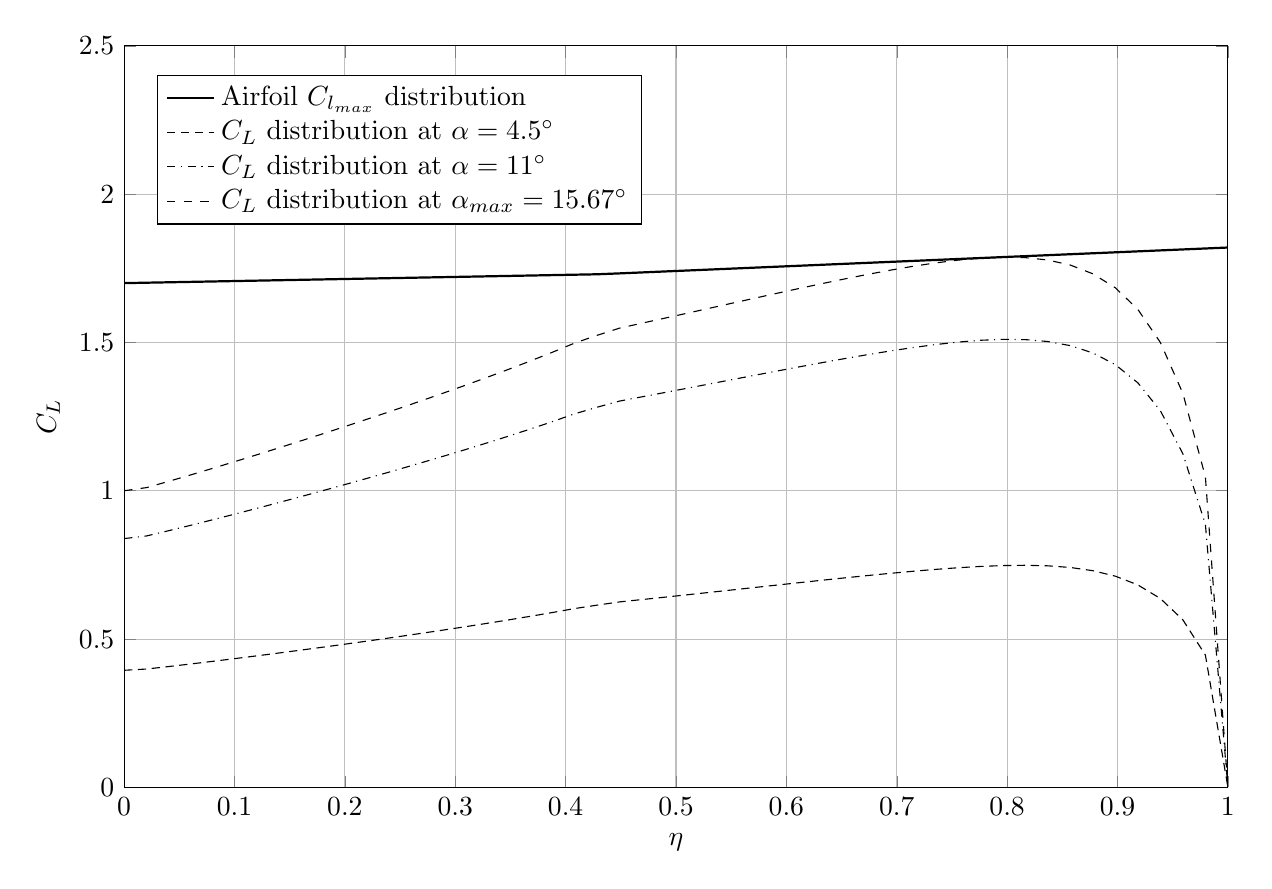
\begin{tikzpicture}
\begin{axis}[
width=15.6cm,
height=11cm,
scaled ticks=false, tick label style={/pgf/number format/fixed},
xmin=0,
xmax=1,
xlabel={$\eta$},
xmajorgrids,
ymin=0,
ymax=2.5,
ylabel={$C_L$ },
ymajorgrids,
legend style={at={(0.03,0.86)},anchor=west,draw=black,fill=white,legend cell align=left},
legend entries = {Airfoil $C_{l_{max}}$ distribution\\$C_L$ distribution at $\alpha = 4.5^{\circ}$\\$C_L$ distribution at $\alpha = 11^{\circ}$\\$C_L$ distribution at $\alpha_{max} = 15.67^{\circ}$\\}
]

\addplot [
color=black,
thick
]
table[row sep=crcr]{
0.0	1.7\\
0.02040816326530612	1.7014205218050096\\
0.04081632653061224	1.7028410436100194\\
0.061224489795918366	1.704261565415029\\
0.08163265306122448	1.705682087220039\\
0.1020408163265306	1.7071026090250485\\
0.12244897959183672	1.7085231308300581\\
0.14285714285714285	1.709943652635068\\
0.16326530612244897	1.7113641744400776\\
0.18367346938775508	1.7127846962450872\\
0.2040816326530612	1.714205218050097\\
0.22448979591836732	1.7156257398551067\\
0.24489795918367344	1.7170462616601165\\
0.26530612244897955	1.7184667834651262\\
0.2857142857142857	1.7198873052701358\\
0.30612244897959184	1.7213078270751456\\
0.326530612244898	1.7227283488801552\\
0.34693877551020413	1.724148870685165\\
0.3673469387755103	1.7255693924901747\\
0.3877551020408164	1.7269899142951843\\
0.40816326530612257	1.7284104361001942\\
0.4285714285714287	1.7298309579052038\\
0.44897959183673486	1.7328438721710124\\
0.469387755102041	1.7360718769054195\\
0.48979591836734715	1.7392998816398264\\
0.5102040816326533	1.7425278863742333\\
0.5306122448979594	1.7457558911086404\\
0.5510204081632656	1.7489838958430473\\
0.5714285714285717	1.7522119005774541\\
0.5918367346938779	1.7554399053118612\\
0.612244897959184	1.758667910046268\\
0.6326530612244902	1.761895914780675\\
0.6530612244897963	1.765123919515082\\
0.6734693877551025	1.768351924249489\\
0.6938775510204086	1.7715799289838958\\
0.7142857142857147	1.774807933718303\\
0.7346938775510209	1.7780359384527098\\
0.755102040816327	1.7812639431871167\\
0.7755102040816332	1.7844919479215238\\
0.7959183673469393	1.7877199526559306\\
0.8163265306122455	1.7909479573903375\\
0.8367346938775516	1.7941759621247446\\
0.8571428571428578	1.7974039668591515\\
0.8775510204081639	1.8006319715935584\\
0.89795918367347	1.8038599763279655\\
0.9183673469387762	1.8070879810623723\\
0.9387755102040823	1.8103159857967792\\
0.9591836734693885	1.8135439905311863\\
0.9795918367346946	1.8167719952655932\\
1.0	1.82\\
};

\addplot [
color=black,
densely dashed
]
table[row sep=crcr]{
0.0	0.39487061827282127\\
0.02040816326530612	0.39911705074252873\\
0.04081632653061224	0.4076541258079028\\
0.061224489795918366	0.41652952400519516\\
0.08163265306122448	0.42565594056919437\\
0.1020408163265306	0.4350003715755874\\
0.12244897959183672	0.44457321126375693\\
0.14285714285714285	0.4543740957294088\\
0.16326530612244897	0.46437786597084324\\
0.18367346938775508	0.4745701097074242\\
0.2040816326530612	0.48494953743854413\\
0.22448979591836732	0.4955213181335934\\
0.24489795918367344	0.5062955525015271\\
0.26530612244897955	0.5172869240067404\\
0.2857142857142857	0.5285149938673958\\
0.30612244897959184	0.5400050288788901\\
0.326530612244898	0.5517894134592906\\
0.34693877551020413	0.5639098643385002\\
0.3673469387755103	0.5764209996551953\\
0.3877551020408164	0.5893967448495923\\
0.40816326530612257	0.6029449006401062\\
0.4285714285714287	0.6145161592513364\\
0.44897959183673486	0.6254249790597856\\
0.469387755102041	0.633360562131451\\
0.48979591836734715	0.6413115057499875\\
0.5102040816326533	0.6493898133875153\\
0.5306122448979594	0.6575566546342706\\
0.5510204081632656	0.6657789548369978\\
0.5714285714285717	0.6740253658806955\\
0.5918367346938779	0.682261993141658\\
0.612244897959184	0.6904498113390178\\
0.6326530612244902	0.6985419656814726\\
0.6530612244897963	0.7064805797604713\\
0.6734693877551025	0.7141927071772669\\
0.6938775510204086	0.7215849857301082\\
0.7142857142857147	0.728536392336933\\
0.7346938775510209	0.734888230846914\\
0.755102040816327	0.740430060576933\\
0.7755102040816332	0.7448795946827579\\
0.7959183673469393	0.747853493711417\\
0.8163265306122455	0.7488241422070676\\
0.8367346938775516	0.7470543487497322\\
0.8571428571428578	0.7414963360881737\\
0.8775510204081639	0.7306311355089603\\
0.89795918367347	0.7122047016299027\\
0.9183673469387762	0.6827747555161765\\
0.9387755102040823	0.6368610861589308\\
0.9591836734693885	0.5649379181298013\\
0.9795918367346946	0.44611515170767324\\
1.0	0.0\\
};

\addplot [
color=black,
dashdotted
]
table[row sep=crcr]{
0.0	0.8387947494521667\\
0.02040816326530612	0.8477767439293765\\
0.04081632653061224	0.8657973942499728\\
0.061224489795918366	0.8844589719269927\\
0.08163265306122448	0.9035670678750508\\
0.1020408163265306	0.9230351964868024\\
0.12244897959183672	0.9428455938058949\\
0.14285714285714285	0.9629840168878613\\
0.16326530612244897	0.9834203626599899\\
0.18367346938775508	1.0041413611645198\\
0.2040816326530612	1.0251513942646675\\
0.22448979591836732	1.046465039224036\\
0.24489795918367344	1.0681052719780921\\
0.26530612244897955	1.0901032642282826\\
0.2857142857142857	1.112499212004902\\
0.30612244897959184	1.135344113861151\\
0.326530612244898	1.1587026503714362\\
0.34693877551020413	1.1826576176874466\\
0.3673469387755103	1.207317018935464\\
0.3877551020408164	1.2328267717969783\\
0.40816326530612257	1.259399727792534\\
0.4285714285714287	1.2816993964991628\\
0.44897959183673486	1.3024481469973197\\
0.469387755102041	1.3168656118879882\\
0.48979591836734715	1.3312017497867599\\
0.5102040816326533	1.3456970300647029\\
0.5306122448979594	1.3602760235105569\\
0.5510204081632656	1.3748752582689432\\
0.5714285714285717	1.3894335435808827\\
0.5918367346938779	1.4038844618781028\\
0.612244897959184	1.4181512936094274\\
0.6326530612244902	1.4321417114914776\\
0.6530612244897963	1.4457414990656257\\
0.6734693877551025	1.4588065789583415\\
0.6938775510204086	1.4711524819152604\\
0.7142857142857147	1.48254007076325\\
0.7346938775510209	1.4926558088105895\\
0.755102040816327	1.5010840253965239\\
0.7755102040816332	1.5072672926971142\\
0.7959183673469393	1.510448850764639\\
0.8163265306122455	1.5095873928752164\\
0.8367346938775516	1.5032283128573634\\
0.8571428571428578	1.4893045161105871\\
0.8775510204081639	1.4648196575519261\\
0.89795918367347	1.4253275780858976\\
0.9183673469387762	1.364038135657163\\
0.9387755102040823	1.2701398312480672\\
0.9591836734693885	1.1248328548451343\\
0.9795918367346946	0.8868495822581037\\
1.0	0.0\\
};

\addplot [
color=black,
dashed
]
table[row sep=crcr]{
0.0	1.0000640627321633\\
0.02040816326530612	1.010766398094911\\
0.04081632653061224	1.0322322534886936\\
0.061224489795918366	1.0544489666798336\\
0.08163265306122448	1.0771832195916318\\
0.1020408163265306	1.10032909772408\\
0.12244897959183672	1.1238586077762809\\
0.14285714285714285	1.1477524648087052\\
0.16326530612244897	1.171978769660344\\
0.18367346938775508	1.1965246673579184\\
0.2040816326530612	1.2213966000647827\\
0.22448979591836732	1.2466125629014233\\
0.24489795918367344	1.272200209131688\\
0.26530612244897955	1.29819670032439\\
0.2857142857142857	1.3246497287501686\\
0.30612244897959184	1.3516196408273637\\
0.326530612244898	1.3791828497184266\\
0.34693877551020413	1.4074370749587437\\
0.3673469387755103	1.436509713439624\\
0.3877551020408164	1.4665728362739583\\
0.40816326530612257	1.4978774579690017\\
0.4285714285714287	1.5240745569055993\\
0.44897959183673486	1.5483979697246268\\
0.469387755102041	1.5651701807448557\\
0.48979591836734715	1.5818259400032437\\
0.5102040816326533	1.598652386123212\\
0.5306122448979594	1.6155607942351458\\
0.5510204081632656	1.63247664975008\\
0.5714285714285717	1.6493279206360283\\
0.5918367346938779	1.6660363743487638\\
0.612244897959184	1.6825115977154743\\
0.6326530612244902	1.698644744149018\\
0.6530612244897963	1.714301129906951\\
0.6734693877551025	1.7293108370663106\\
0.6938775510204086	1.7434562988887734\\
0.7142857142857147	1.7564554695665604\\
0.7346938775510209	1.767938561742706\\
0.755102040816327	1.777415348553641\\
0.7755102040816332	1.7842284486163926\\
0.7959183673469393	1.7874854453191305\\
0.8163265306122455	1.7859584175320053\\
0.8367346938775516	1.7779321357558397\\
0.8571428571428578	1.7609692065093554\\
0.8775510204081639	1.7315365815753476\\
0.89795918367347	1.6843917480484274\\
0.9183673469387762	1.6115283479740061\\
0.9387755102040823	1.5001981253624803\\
0.9591836734693885	1.3282321873237517\\
0.9795918367346946	1.046960137106503\\
1.0	0.0\\
};
\end{axis}
\end{tikzpicture}%

\caption{BOEING 747-100B Stall Path at Mach 0.84.}
\label{fig:stallB}
\end{figure}


\begin{center}
\captionof{table}{High-lift devices geometrical data for BOEING 747-100B. Flap.}
	\begin{tabular}{| l | l | l | l | l |}
		\hline
		 Number of Flap & Type &  $\eta$ in &  $\eta$ out &   $\frac{c_{f}}{c} $  \\ \hline
				1  & Triple Slotted&  0.104  & 0.357  & 0.18 \\ \hline 
		         2& Triple Slotted & 0.411 & 0.636 &0.18\\ \hline 
		\hline
	\end{tabular}
\end{center}


\begin{center}
\captionof{table}{High-lift devices geometrical data for BOEING 747-100B. Slat.}
	\begin{tabular}{| l | l | l | l | l |}
		\hline
		 Number of Slat &  $\eta$ in &  $\eta$ out &   $\frac{c_{ext}}{c} $ & $\frac{c_{s}}{c} $   \\ \hline
				1 & 0.192  & 0.364  &1.1 & 0.09\\ \hline 
		         2 & 0.414  & 0.648  &1.1& 0.136\\ \hline 
		         3 & 0.692  & 0.961  &1.1& 0.187\\ \hline 
		\hline
	\end{tabular}
\end{center}


\begin{center}
\captionof{table}{High-lift devices data for  BOEING 747-100B}
	\begin{tabular}{ | l | l | l | l | l | l |}
		\hline
		Configuration &  $\delta_{f_1}$ & $\delta_{f_2}$ &  $\delta_{s_1}$ & $\delta_{s_2}$& $\delta_{s_3}$ \\ \hline
		Take off &  $5^{\circ}$, $3^{\circ}$, $2^{\circ}$ & $5^{\circ}$, $3^{\circ}$, $2^{\circ}$ & $10^{\circ}$ &  $10^{\circ}$ &  $10^{\circ}$\\ \hline
		Landing  &    $10^{\circ}$, $10^{\circ}$, $10^{\circ}$ & $10^{\circ}$, $10^{\circ}$, $10^{\circ}$ & $20^{\circ}$ &  $20^{\circ}$ &  $20^{\circ}$\\ \hline
		\hline
	\end{tabular}
\end{center}


\begin{figure}[H]
\centering
%CL alpha Wing High Lift
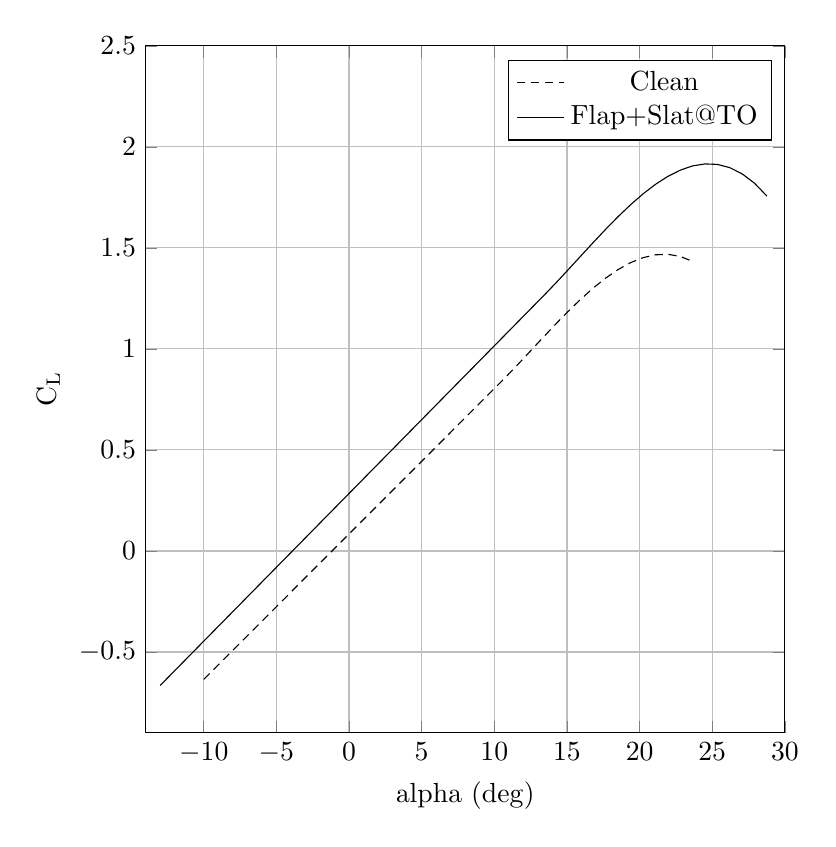
\begin{tikzpicture}

\begin{axis}[
width=0.8\textwidth,
height=0.85\textwidth,
scaled ticks=false, tick label style={/pgf/number format/fixed},
xmin=-14.0,
xmax=30,
xlabel={alpha ($\deg$)},
xmajorgrids,
ymin=-0.9,
ymax=2.5,
ylabel={C\textsubscript{L}},
ymajorgrids,
legend entries = {Clean\\Flap+Slat@TO\\}
]

\addplot [
color=black,
densely dashed
]
table[row sep=crcr]{
-10.0	-0.6352658757762881\\
-9.136225640983186	-0.5731327253055505\\
-8.272451281966372	-0.5109995748348128\\
-7.4086769229495575	-0.4488664243640752\\
-6.544902563932743	-0.3867332738933375\\
-5.681128204915928	-0.32460012342259975\\
-4.817353845899113	-0.2624669729518621\\
-3.9535794868822984	-0.2003338224811243\\
-3.0898051278654837	-0.13820067201038666\\
-2.226030768848669	-0.07606752153964896\\
-1.3622564098318544	-0.013934371068911253\\
-0.4984820508150398	0.04819877940182644\\
0.3652923082017747	0.11033192987256413\\
1.2290666672185893	0.17246508034330182\\
2.092841026235404	0.23459823081403952\\
2.956615385252219	0.2967313812847773\\
3.8203897442690335	0.3588645317555149\\
4.684164103285848	0.42099768222625267\\
5.547938462302663	0.4831308326969903\\
6.411712821319478	0.5452639831677281\\
7.275487180336293	0.6073971336384656\\
8.139261539353107	0.6695302841092035\\
9.003035898369921	0.7316634345799412\\
9.866810257386735	0.7937965850506788\\
10.730584616403549	0.8562885913586846\\
11.594358975420363	0.9210695330328473\\
12.458133334437177	0.9874024124846988\\
13.32190769345399	1.0540582567871901\\
14.185682052470804	1.1198080930132723\\
15.049456411487618	1.183422948235896\\
15.913230770504432	1.2436738495280117\\
16.777005129521246	1.2993318239625704\\
17.64077948853806	1.3491678986125228\\
18.504553847554877	1.3919531005508203\\
19.368328206571693	1.4264584568504133\\
20.23210256558851	1.4514549945842523\\
21.095876924605324	1.46571374082529\\
21.95965128362214	1.4680057226464747\\
22.823425642638956	1.4571019671207581\\
23.687200001655764	1.4317735013210915\\
};

\addplot [
color=black,
solid
]
table[row sep=crcr]{
-13.0	-0.6656753795627666\\
-12.147624487600394	-0.6033806637646808\\
-11.295248975200789	-0.5410859479665948\\
-10.442873462801183	-0.4787912321685088\\
-9.590497950401577	-0.416496516370423\\
-8.738122438001971	-0.354201800572337\\
-7.885746925602365	-0.29190708477425126\\
-7.033371413202758	-0.22961236897616527\\
-6.180995900803151	-0.16731765317807928\\
-5.328620388403545	-0.10502293737999341\\
-4.476244876003938	-0.04272822158190742\\
-3.623869363604332	0.019566494216178454\\
-2.771493851204726	0.08186121001426439\\
-1.9191183388051196	0.14415592581235026\\
-1.0667428264055134	0.2064506416104362\\
-0.21436731400590714	0.2687453574085221\\
0.6380081983936992	0.331040073206608\\
1.4903837107933056	0.39333478900469393\\
2.3427592231929117	0.45562950480277986\\
3.195134735592518	0.5179242206008657\\
4.0475102479921246	0.5802189363989516\\
4.899885760391731	0.6425136521970376\\
5.752261272791338	0.7048083679951236\\
6.604636785190944	0.7671030837932096\\
7.457012297590551	0.8293977995912953\\
8.309387809990158	0.8916925153893813\\
9.161763322389763	0.9539872311874671\\
10.01413883478937	1.016281946985553\\
10.866514347188975	1.0785766627836388\\
11.71888985958858	1.1408713785817248\\
12.571265371988186	1.2031660943798108\\
13.423640884387792	1.2654622144570093\\
14.276016396787398	1.3292987998867514\\
15.128391909187004	1.3952270046956958\\
15.98076742158661	1.462047574490369\\
16.833142933986217	1.5285612548772958\\
17.685518446385824	1.5935687914630023\\
18.537893958785432	1.655870929854015\\
19.39026947118504	1.71426841565686\\
20.242644983584647	1.767561994478062\\
21.095020495984254	1.8145524119241483\\
21.947396008383862	1.8540404136016424\\
22.79977152078347	1.884826745117074\\
23.652147033183077	1.9057121520769658\\
24.504522545582685	1.9154973800878456\\
25.356898057982292	1.9129831747562378\\
26.2092735703819	1.8969702816886713\\
27.061649082781507	1.8662594464916673\\
27.914024595181115	1.8196514147717553\\
28.766400107580708	1.7559469321354586\\
};
\end{axis}
\end{tikzpicture}%

\caption{BOEING 747-100B  lift curve with and without flaps in take-off configuration.}
\label{fig:clATR}
\end{figure}

\begin{lstlisting}[caption={{\footnotesize Wing Lift characteristic results for TAKE-OFF. BOEING 747-100B, M=0.2 }},label= [style=\bfseries]{Listing}]


-----------CLEAN-------------- 
 alpha max 21.1765973230843 (deg)
 alpha star 9.7482928348910 (deg)
 cl max 1.4597134105954703
 cl star 0.8130642471456172
 cl alpha 4.121408852511737 (1/rad)


 ----------- DELTA HIGH LIFT TAKE_OFF-------------- 
deltaCL0_flap = 0.5985742466275841
deltaCLmax_flap = 0.6272563565428977
deltaCLmax_slat = 0.0
cLalpha_new = (1/rad) 4.153009870215378
deltaAlphaMax = (deg) 2.4385950909414857
deltaCD = 0.023580578759700432
deltaCMc_4 = -0.12074049808439227


 -----------HIGH LIFT-------------- 
 alpha max 21.431119618227623 (deg)
 alpha star 10.003551951328152 (deg)
 cl max 2.086969767138368
 cl star 1.4354638015005163
 cl alpha 4.153009870215378 (1/rad)
 
 CL of wing at TAKE_OFF at alpha body 2 (deg) = 0.9641157258005986
\end{lstlisting}

\section{Modified Stall Path}

In order to evaluate the lift curve of a wing another method has been implemented. This is a modification of Stall Path Method that uses the Nasa-Blackwell lift distribution also for the non linear trait. As known NB method does not see the viscous phenomena. The modified stall path method is based on the consideration that the lift distribution obtained from Nasa-Blackwell is the distribution that you would get if the airfoil's lift moved along the linear lift curve.\\
The process is the following.

\begin{enumerate}
	\item For each angle of attack the lift distribution using Nasa-Blackwell method has been evaluated
	\item For each of n point along the semi-span the local value of $C_L$ is obtained 
	\item Each of these n points corresponds to an intermediate airfoil with its own lift curve
	\item With the local value of $C_l$  it is possible to enter in the linear lift chart obtaining the angle of attack of the airfoil
	\item Using this angle of attack it is possible to enter in the lift curve of the airfoil and derive the local $C_l$
	\item In this way a new lift distribution is obtained that considers the bidimensional non linearity.
	\item The wing $C_L$ is obtained integrating the new lift distribution.
\end{enumerate}

\begin{figure}[H]
	\centering
	{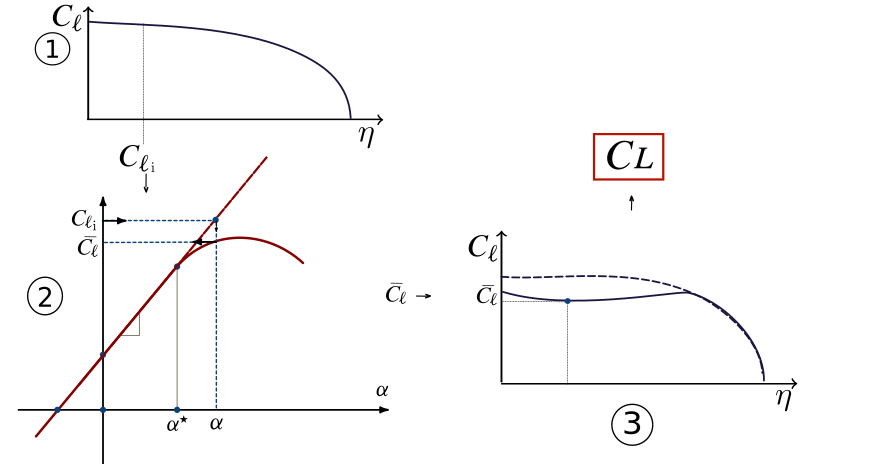
\includegraphics[height=9 cm]{Immagini/stallpathmodified.pdf}} 
	\caption{Flow chart of the modified stall path method.}
	\label{fig:spmm}
\end{figure}

\section{Results Comparison}
In order to compare and validate the results an analysis on a wing has been done with different method.

\begin{center}
\captionof{table}{Airfoils Data}
	\begin{tabular}{| l | l | l | l | l |}
		\hline
		 Station & t/c & $C_{l_{max}}$ & $C_{l_{\alpha}}$ & $\alpha_{stall}$ \\ \hline
		 Root & $0.18$ &  1.90  &  $6.48 (1/rad)$ & $ 18^{\circ} $  \\ \hline
		 Kink & $0.18$ & 1.90  &  $6.48 (1/rad)$ & $ 18^{\circ} $  \\ \hline
		 Tip & $0.18$ &  2.1  &  $6.72 (1/rad)$ & $ 17.5^{\circ} $  \\ \hline
		\hline
	\end{tabular}
\end{center}
\begin{center}
\captionof{table}{Wing Data}
	\begin{tabular}{| l | l | l | l | l |  l |}
		\hline
		  Span & Aspect Ratio & Cr & Ck & Cr & Ad. station kink  \\ \hline
		  31  m & 12 & 2.9 m & 2.9 m & 1.65 m & 0.33\\ \hline
		\hline
	\end{tabular}
\end{center}
\begin{center}
\captionof{table}{Mission Data}
	\begin{tabular}{| l | l |}
		\hline
		  Reynolds Number & Mach Number\\ \hline
		  $13 \cdot 10^6$  & 0.2   \\ \hline
		\hline
	\end{tabular}
\end{center}


The analysis has been done with the following methods :

\begin{itemize}
\item Stall Path
\item Modified Stall Path
\item Philipps and Alley
\item CFD
\end{itemize}

{\bfseries Phillips and Alley} present a method for estimating the maximum wing lift that is based on the classical lifting line theory discussed in Appendix C. Their approach involves providing correction factors for the effects of twist and sweep-back on the span loading of unswept, untwisted, tapered wings. The correction factors are developed with the aid of CFD panel method computations for a variety of conventional wing planforms. Curves for the correction factors are presented for a number of specific taper and aspect ratio as long with the general method for calculating these effects for other wing geometry. \cite{sforza2014commercial}

\begin{equation}
C_{L_{max}} = \left ( \frac{C_L}{c_{l_{max}}}\right)_{\Gamma =0 , \epsilon =0} K_{LS} K_{L\Gamma c_{l_{max}}} \left ( 1 - \frac { K_{L \epsilon} C_{L,\alpha \epsilon}}{c_{l_{max}}} \right) 
\end{equation}

Where $K_{LS}$ is a stall factor

\begin{equation}
K_{LS}=1 + (0.0042 \AR -0.066) \left (1+2.3 \frac{C_{L_{\alpha}}}{ c_{l_{max}}} \right )
\end{equation}

\noindent \\
{\bfseries Computational Fluid Dynamics (CFD)} is a methodology that allows engineers to predict the performance of their designs when exposed to fluid flow, either internal flow (such as the flow of air and gasoline through an engine manifold) or external flow (such as the aerodynamic flow past an automobile or the hydrodynamic flow past a boat). CFD software programs can simulate problems involving gases, liquids and solids and multi-phase problems that depend on the interaction of any number of the above. CFD is used in the design of almost every major product, reducing uncertainty in the design process, and resulting in higher quality products and designs, with greater robustness that better meet customer requirements. CD-adapco is the world's largest independent CFD focused provider of engineering simulation software, support and services. \cite{adapco} \\ \\
Considering the reduction of $CL_{max}$ due to flow separation and other tridimensional effects, an additional modification has been implemented starting from the Stall Path method and the Modified Stall Path Method. The used value for $CL_{max}$ is obtained from the traditional Stall Path method, while the value of $\alpha_{max}$ is obtained from the modified Stall Path Method. In this way a small percentual error has been obtained.


\begin{figure}[H]
	\centering
	{\includegraphics[height=4.9 cm]{Immagini/comparisonairfoil.png}} 
	\caption{Comparison of wing lift curve of airfoils.}
	\label{fig:met}
\end{figure}
	 	 
\noindent \\

	 	 
\begin{figure}[H]
	\centering
	{\includegraphics[height=9.9 cm]{Immagini/clmaxcomparison1.png}} 
	\caption{Comparison of wing lift curve of wing.}
	\label{fig:met}
\end{figure}
	 	 
	 	 
\noindent \\
\begin{center}
\captionof{table}{Lift results comparison}
	\begin{tabular}{| l | l | l | }
		\hline
		 Method  & $C_{L_{MAX}}$ & $\alpha_{stall}$   \\ \hline
		 Stall Path  &1.766  & $17.1 ^{\circ}$  \\ \hline
		 Modified Stall Path  & 1.86   & $19.5^{\circ}$  \\ \hline
		 Modified Stall Path II  & 1.766  & $19.5^{\circ}$  \\ \hline
		 Phillips And Alley  & 1.83  & n.e.\\ \hline
		 CFD  & 1.699  & $19.6 ^{\circ}$   \\ \hline
		\hline
	\end{tabular}
\end{center}

\begin{figure}[H]
	\centering
	{\includegraphics[height=2.63cm]{Immagini/referencepercent.png}} 
	\caption{Percentage Error.}
	\label{fig:met}
\end{figure}

